\documentclass[border=10pt]{standalone}

\usepackage{tikz}
\usepackage{tikzsymbols}
\usetikzlibrary{calc,patterns,shapes.geometric}

\def\centerarc[#1](#2)(#3:#4:#5){\draw[#1] ($(#2)+({#5*cos(#3)},{#5*sin(#3)})$) arc (#3:#4:#5);}

\begin{document}
	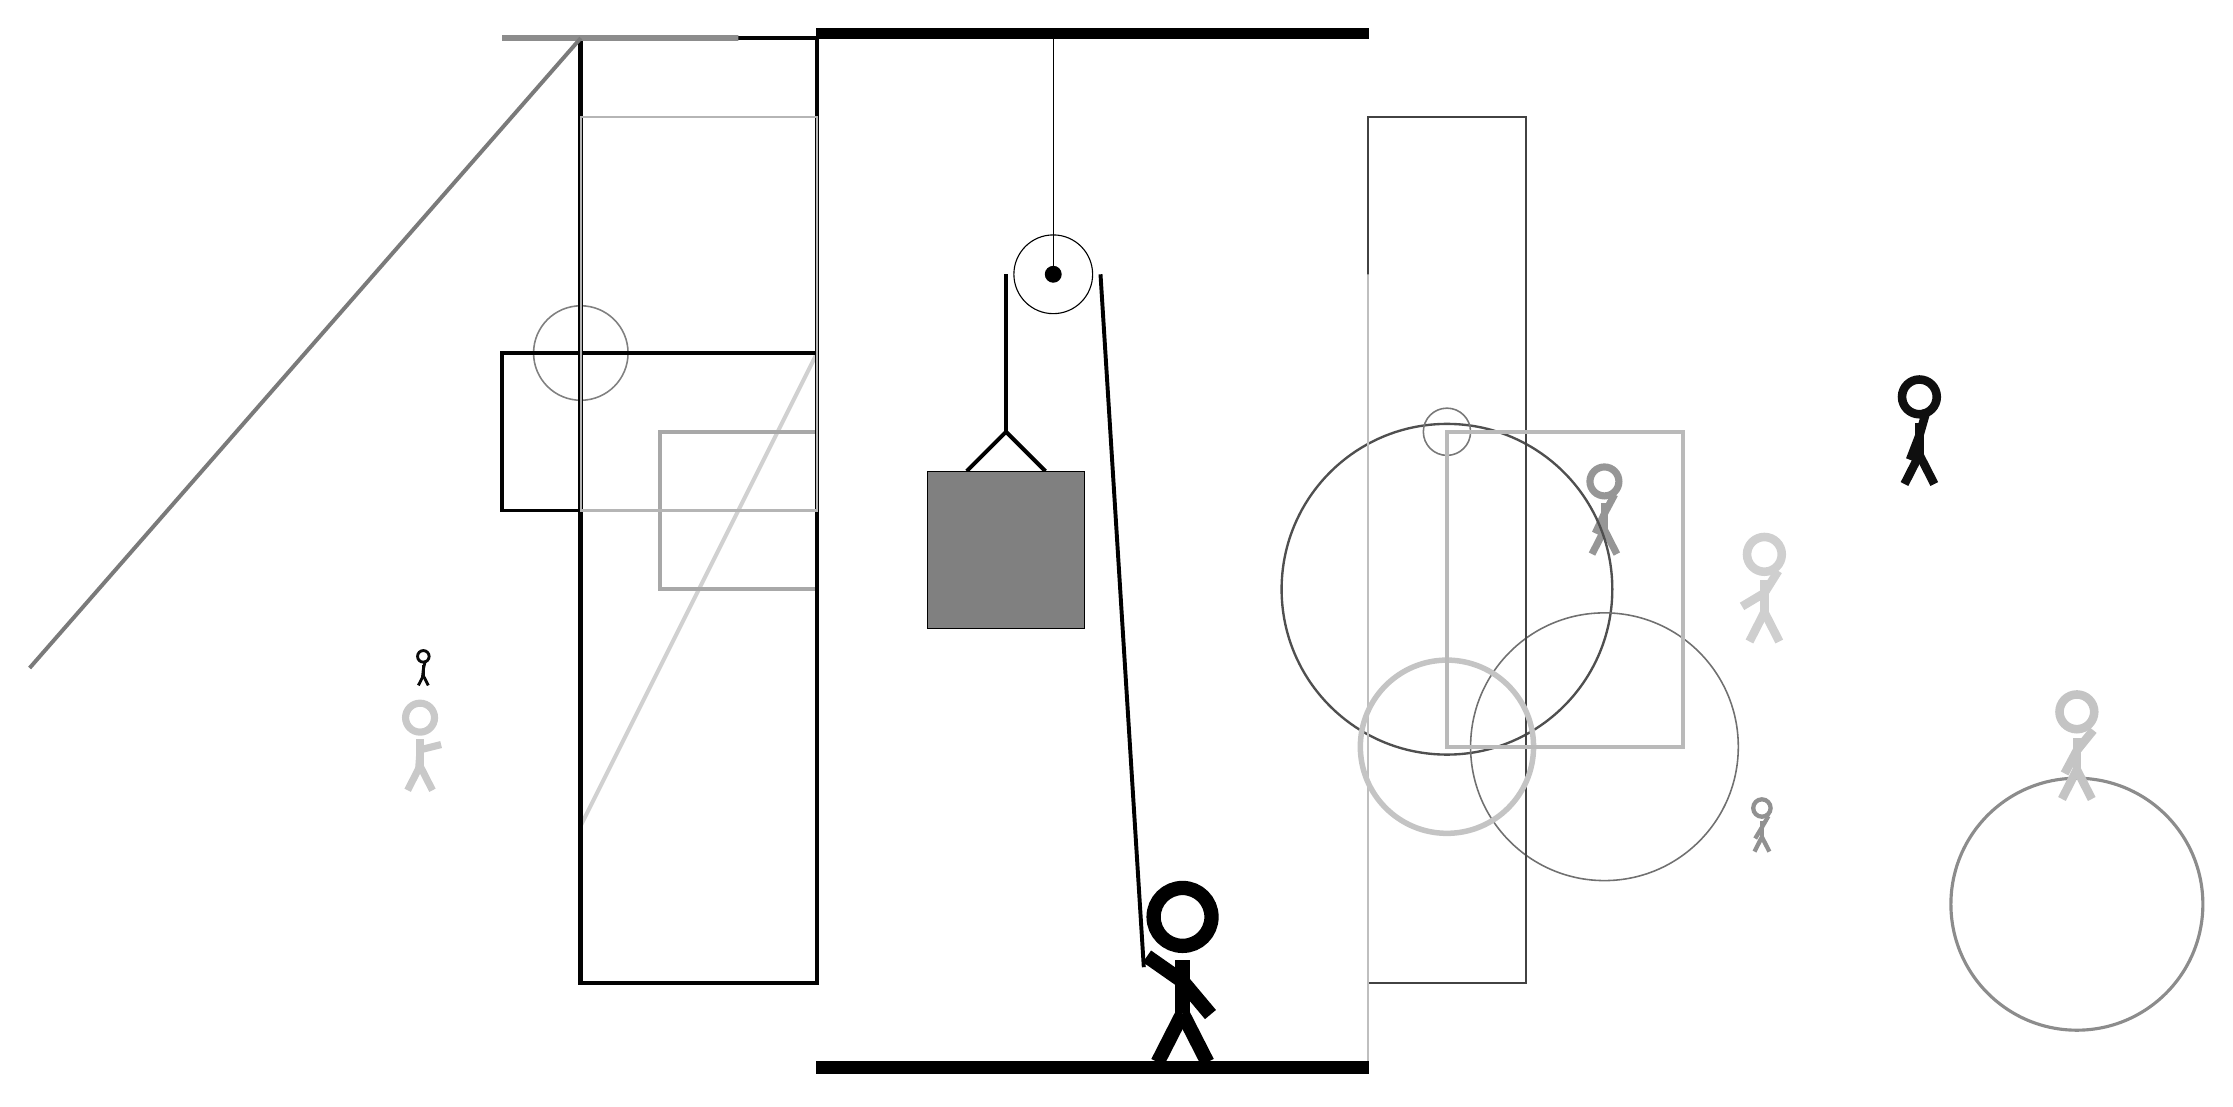
\begin{tikzpicture}
		%%%%% START %%%%%
		
		\draw[fill=black] (-2, 10) rectangle (5, 10.125);
		
		\draw (1, 7) circle (0.5);
		\draw[fill=black] (1, 7) circle (0.1);
		\draw (1, 10) -- (1, 7);
		
		\node[line width=0.3mm, color=black!21] at (-7, 1) {\Strichmaxerl[5][86][14]};
		
		\draw[line width=0.5mm, color=black!18](-5, 0) -- (-2, 6);
		\node[line width=0.3mm, color=black!41] at (8, 4) {\Strichmaxerl[5][65][62]};
		\draw [line width=0.3mm, color=black!69](6, 3) circle (2.1);
		
		\draw [line width=0.2mm, color=black!50](-5, 6) circle (0.6);
		
		\draw[line width=0.5mm, color=black!99] (-2, 4) rectangle (-6, 6);
		\draw [line width=0.2mm, color=black!53](6, 5) circle (0.3);
		\draw [line width=0.2mm, color=black!56](8, 1) circle (1.7);
		\draw[line width=0.5mm, color=black!67](-2, 4) -- (-2, 10);
		\draw[line width=0.2mm, color=black!74] (5, -2) rectangle (7, 9);
		\node[line width=0.3mm, color=black!94] at (12, 5) {\Strichmaxerl[6][69][74]};
		
		\draw[line width=0.5mm, color=black!34] (-4, 3) rectangle (-2, 5);
		\draw[line width=0.3mm, color=black!25] (5, 7) rectangle (5, -3);
		
		\draw [line width=0.4mm, color=black!45](14, -1) circle (1.6);
		\node[line width=0.5mm, color=black!19] at (10, 3) {\Strichmaxerl[6][31][58]};
		\draw[line width=0.6mm, color=black!99] (-2, 10) rectangle (-5, -2);
		
		\draw[line width=0.7mm, color=black!45] (-3, 10) rectangle (-6, 10);
		\draw [line width=0.7mm, color=black!23](6, 1) circle (1.1);
		\node[line width=0.4mm, color=black!43] at (10, 0) {\Strichmaxerl[3][59][60]};
		\node[line width=0.3mm, color=black!23] at (14, 1) {\Strichmaxerl[6][62][51]};
		\draw[line width=0.3mm, color=black!29] (-2, 9) rectangle (-5, 4);
		
		\draw[line width=0.5mm, color=black!27] (6, 5) rectangle (9, 1);
		\draw[line width=0.5mm, color=black!52](-5, 10) -- (-12, 2);
		\node[line width=0.7mm, color=black!96] at (-7, 2) {\Strichmaxerl[2][84][77]};
		
		\draw[line width=0.5mm] (-0.1, 4.5) -- (0.4, 5.0) -- (0.9, 4.5);
		\draw[fill=black!50] (-0.6, 4.5) rectangle (1.4, 2.5);
		
		\draw[line width=0.5mm] (0.4, 7) -- (0.4, 5.0);
		\centerarc[line width=0.5mm](1, 7)(0:180:0.6);
		\draw[line width=0.5mm](1.6, 7) -- (2.15, -1.8);
		
		\node at (2.6, -1.9) {\Strichmaxerl[10][-35][-50]};
		
		\draw[fill=black] (-2, -3) rectangle (5, -3.15);
		
		%%%%% END %%%%%
	\end{tikzpicture}
\end{document}